La sezione \emph{Configurazione Prometheus} (cfr. sezione \ref{prometheus}) selezionabile dal menu consente all'utente due operazioni essenziali:

\begin{enumerate}[noitemsep,nolistsep]
    \item Caricare una nuova configurazione Prometheus
    \item Visualizzare lo stato corrente della Prometheus
\end{enumerate}

\begin{figure}[H]
    \begin{center}
    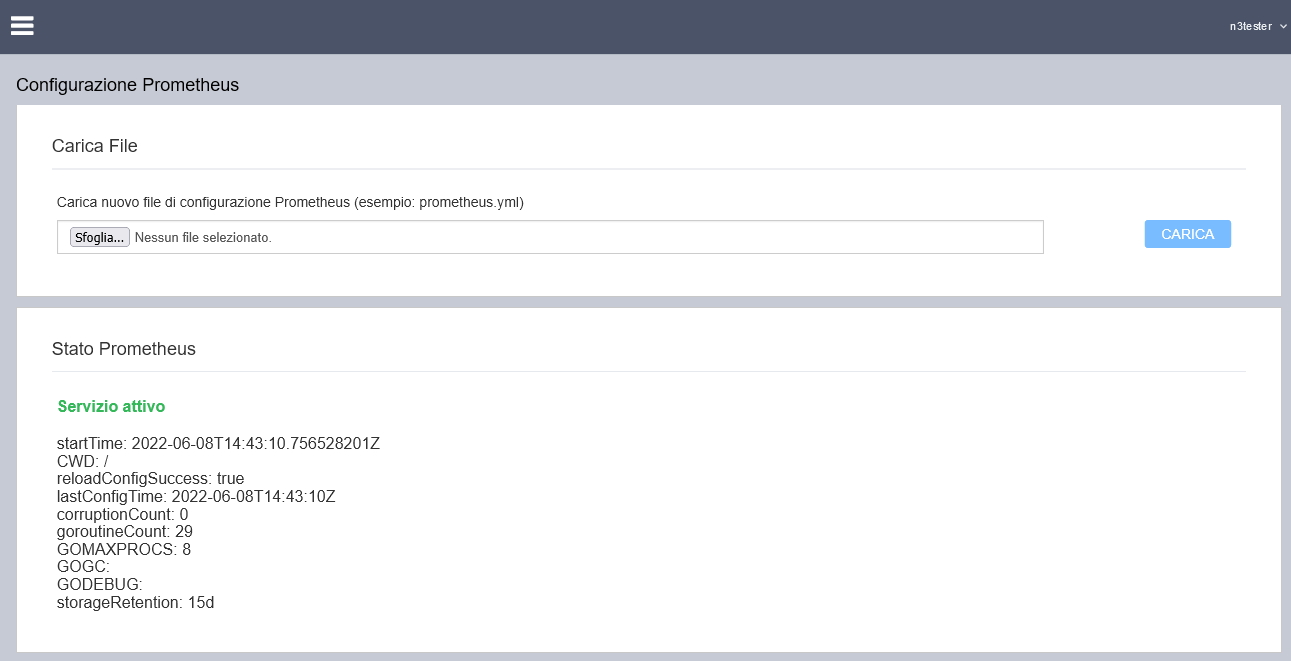
\includegraphics[width=\textwidth]{images/full-prometheus.png}
    \caption{Sezione \emph{Configurazione Prometheus}.}
    \end{center}
\end{figure}

\subsection{Caricamento nuova configurazione}

L'utente può caricare, in modo analogo alla sezione relativa alla VPN, un nuovo file di \textbf{configurazione Prometheus}, in formato \textbf{YML}. 

Ugualmente alla configurazione OpenVPN, il server al momento della ricezione del nuovo file, \textbf{accede in SSH} all'host dal container (cfr. sezione \ref{fig:containers-arch}); successivamente copia con SCP il nuovo file di configurazione e \textbf{riavvia il service Prometheus}.

\begin{figure}[H]
    \begin{center}
    
\includegraphics[width=\textwidth]{images/prometheus-file.png}
    \caption{Sezione per il caricamento di un nuovo file di configurazione OpenVPN.}
    \end{center}
\end{figure}

\subsection{Visualizzazione stato corrente Prometheus}

Come per la VPN, anche per Prometheus l'utente ha la facoltà di visualizzare lo \textbf{stato corrente} del servizio.

\begin{figure}[H]
    \begin{center}
    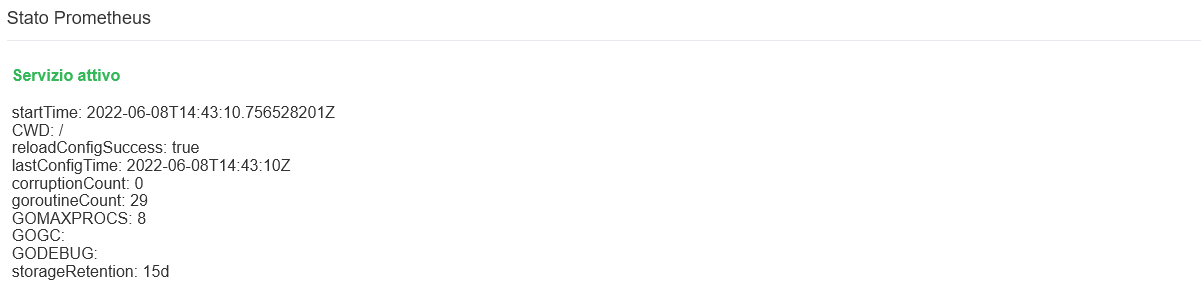
\includegraphics[width=\textwidth]{images/prometheus-status.png}
    \caption{Stato corrente Prometheus.}
    \end{center}
\end{figure}

La web application ricava lo stato di Prometheus direttamente dal client facendo una \emph{request} all'endpoint predefinito dal servizio:\\
\texttt{http://<hostname>:9090/api/v1/status/runtimeinfo}